%%%%%%%%%% NO OLVIDAR COLOCAR ESTE COMENTARIO CON EL NUMERO DE EJERCICIO %%%%%%%%%%%%%
%%%%%%%%%%%%%%%%%%% EJERCICIO 5 %%%%%%
%%Text bf para negrilla , el \\ es para el salto de linea.
%%El primer \\ hace un espacio en el texto y el 2 \\ crea otro espacio
	\textbf{Ejemplo 4}\newline
	Una persona arrienda una casa en 50.000 COP pagaderos por mes anticipado, Si tan pronto como recibe cada arriendo, lo invierte en un fondo que le paga el 2\% periodo mes anticipado ¿Cuál será el monto de sus ahorros al final de un año?\\ \\

	\textbf{Solución.}\\
	\begin{center}

		\renewcommand{\arraystretch}{1.5}% Margenes de las celdas
		%Creación de la cuadricula
		\begin{longtable}{|c|c|c| }
			%Creamos una linea horizontal
			\hline
			%Definimos el color de la primera fila
			\rowcolor[HTML]{FFB183}
			%%%%% INICIO ASIGNACIÓN FECHA FOCAL %%%%%%%
			%%%%%%%%%% INICIO TITULO
			%Lo que se hace aquí es mezclar las 3 columnas en una sola
			\multicolumn{3}{|c|}{\cellcolor[HTML]{FFB183}\textbf{1. Asignación período focal}}   \\ \hline
			%%%%%%%%%% FIN TITULO
			%%%%% INICIO DECLARACIÓN DE VARIABLES %%%%%%%
			\multicolumn{3}{|c|}{$pf = 12pma$} \\ \hline
			%Definimos el color de la primera fila
			\rowcolor[HTML]{FFB183}
			%%%%% INICIO DECLARACIÓN DE VARIABLES %%%%%%%
			%%%%%%%%%% INICIO TITULO
			\multicolumn{3}{|c|}{\cellcolor[HTML]{FFB183}\textbf{2. Declaración de variables}}                                                                                   \\ \hline
			%%%%%%%%%% FIN TITULO
			%%%%%%%%%% INICIO DE MATEMÁTICAS
			R = 50.000 COP  & $n = 12 pma$  &	i=2\% pma  \\ \hline
			\multicolumn{3}{|c|}{VF = ? COP} \\ \hline
			%%%%%%%%%% FIN DE MATEMÁTICAS
			%%%%% FIN DECLARACIÓN DE VARIABLES


			%%%%% INICIO FLUJO DE CAJA
			\rowcolor[HTML]{FFB183}
			\multicolumn{3}{|c|}{\cellcolor[HTML]{FFB183}\textbf{3. Diagrama de flujo de caja}}                                                                                  \\ \hline
			%Mezclamos 3 columnas y pondremos el dibujo
			%%%%%%%%%%%%% INSERCIÓN DE LA IMAGEN
			\multicolumn{3}{|c|}{ 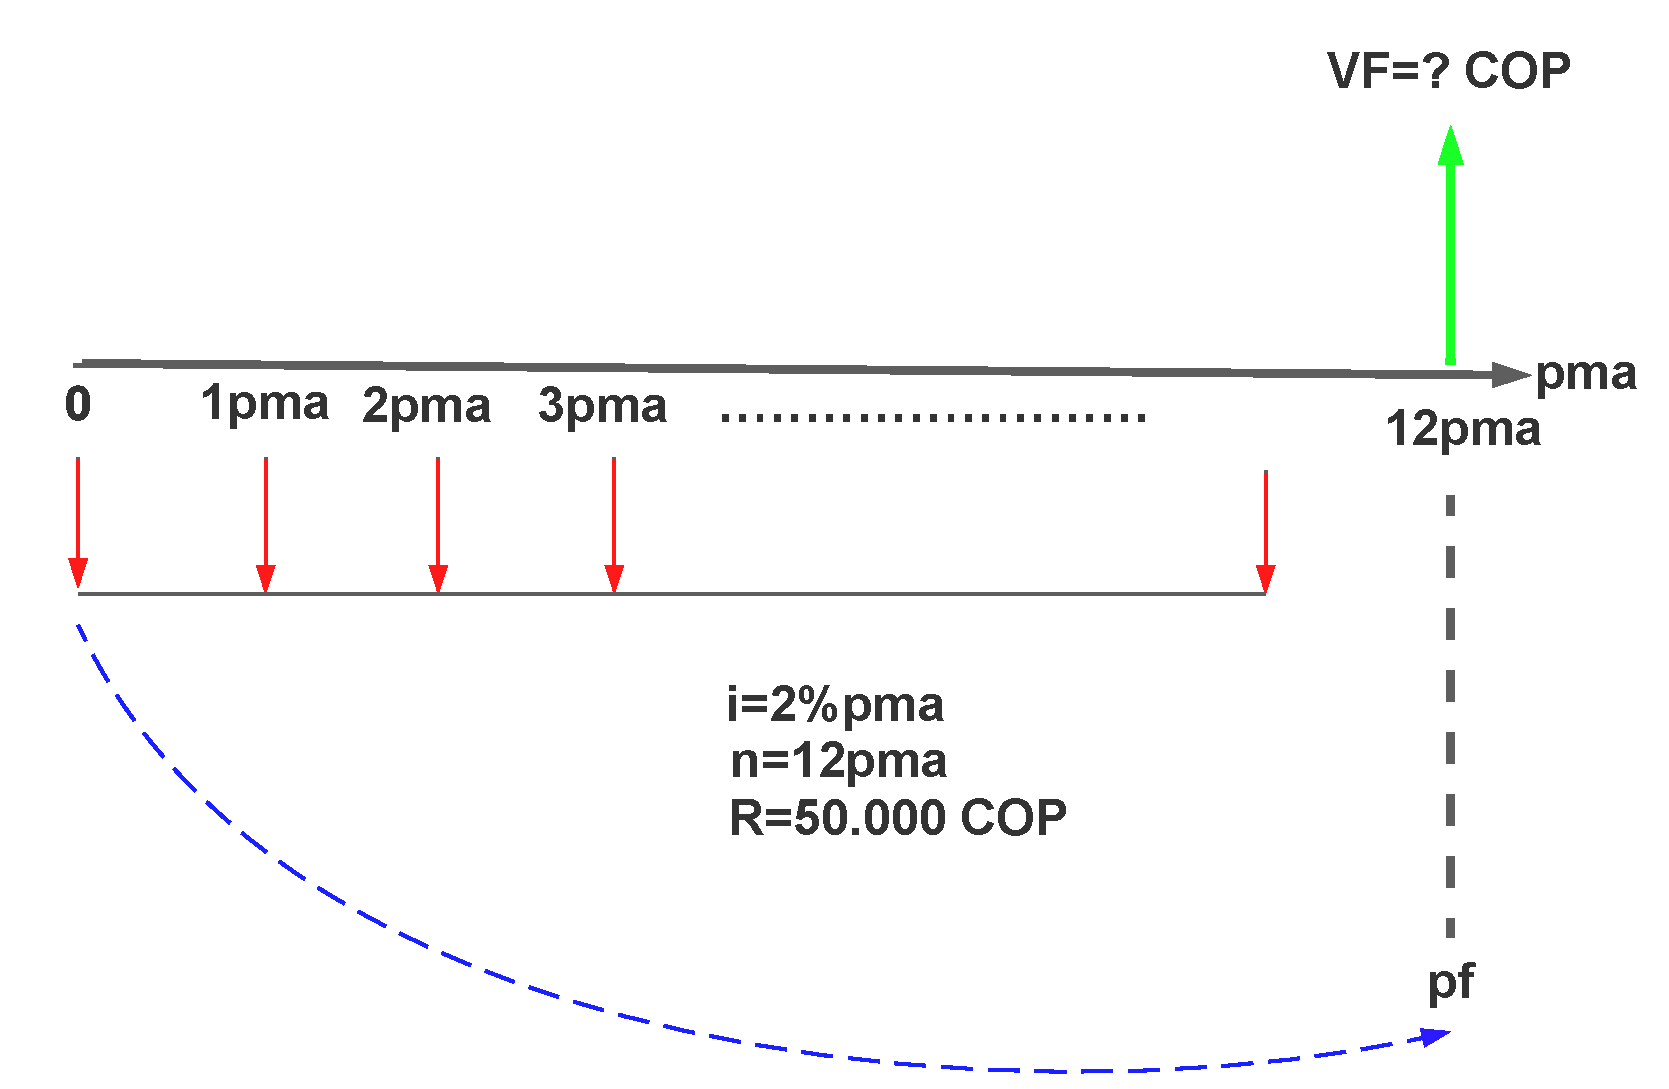
\includegraphics[scale=0.5]{4_Capitulo/img/ejemplos/5/capitulo4ejemplo5.pdf} }                                                                                         \\ \hline
			%%%%%%%%%%%%% FIN INSERCIÓN DE IMAGEN
			%%%%%FIN FLUJO DE CAJA



			%%%%% INICIO DECLARACIÓN FORMULAS
			%%%%%%%%%%% INICIO TITULO
			\rowcolor[HTML]{FFB183}
			\multicolumn{3}{|c|}{\cellcolor[HTML]{FFB183}\textbf{4. Declaración de fórmulas}}                                                                                    \\ \hline
			%%%%%%%%%%% FIN TITULO
			%%%%%%%%%%% INICIO MATEMÁTICAS

			 \multicolumn{3}{|c|}{$VF_a=R \frac{(1+i)^{n}-1}{i}(1+i)$ \hspace{0.3cm} \textit{Valor futuro serie uniforme anticipada}}                                                           \\ \hline
			%%%%%%%%%% FIN MATEMÁTICAS
			%%%%%% INICIO DESARROLLO MATEMÁTICO
			\rowcolor[HTML]{FFB183}
			%%%%%%%%%%INICIO TITULO
			\multicolumn{3}{|c|}{\cellcolor[HTML]{FFB183}\textbf{5. Desarrollo matemático}}                                                                                      \\ \hline
			%%%%%%%%%% FIN TITULO
			%%%%%%%%%% INICIO MATEMÁTICAS
			\multicolumn{3}{|c|}{$VF_{a}=$50.000 COP$\frac{(1+0,02)^{12}-1}{0,02}(1+0,02)=$684.016,58 COP}                               \\ \hline
			%%%%%%%%%% FIN MATEMÁTICAS
			%%%%%% FIN DESARROLLO MATEMÁTICO

			\rowcolor[HTML]{FFB183}
			\multicolumn{3}{|c|}{\cellcolor[HTML]{FFB183}\textbf{6. Respuesta}}    \\ \hline

			\multicolumn{3}{|c|}{El monto de sus ahorros al final de año será de 684.017 COP} \\ \hline
		\end{longtable}
		%Se crean dos lineas en blanco para que no quede el siguiente texto tan pegado
		%\newline \newline
	\end{center}
%%%%%%%%%%%%%%%%%%%%%%%%%%FIN EJERCICIO X %%%%%%%%%%%%%%%%%%%%%%%%%%%
